% Real Matching along Curved Paths: From the Line to the Classroom Tour
% VISGRAF Lab technical note. 22 November 2026.
% Build: pdflatex curved.tex twice, in this folder (or Overleaf with this file as the main document).
% Figures in figs/ come from the records of visgraf/deep-motion (figs/SOURCES.md).
\documentclass[11pt,a4paper]{article}

\usepackage[T1]{fontenc}
\usepackage[utf8]{inputenc}
\IfFileExists{lmodern.sty}{\usepackage{lmodern}\usepackage{microtype}}{\usepackage[expansion=false]{microtype}}
\usepackage[a4paper,top=2.5cm,bottom=2.6cm,left=2.6cm,right=2.6cm]{geometry}
\usepackage{textcomp}
\usepackage{amsmath,amssymb}
\usepackage{booktabs}
\usepackage{tabularx}
\usepackage{array}
\usepackage{xcolor}
\usepackage{enumitem}
\usepackage{graphicx}
\usepackage[font=small,labelfont=bf]{caption}
\usepackage{placeins}
\usepackage[hidelinks]{hyperref}
\hypersetup{colorlinks=true,linkcolor=black!70!blue,citecolor=black!70!blue,urlcolor=black!70!blue,
  pdftitle={Real Matching along Curved Paths: From the Line to the Classroom Tour},
  pdfauthor={Luiz Velho, with Claude (Anthropic)},
  pdfsubject={VISGRAF technical note, 22 November 2026}}
% figures resolve whether the compile runs in this folder or at the repository's root
\graphicspath{{figs/}{curved-paths/figs/}}

% ---------------------------------------------------------------- VISGRAF cover
\IfFileExists{techrep-ic.sty}{%
  \usepackage{techrep-ic}%
  \newcommand{\MakeVisgrafCover}{%
    \TRNumber{19}   % <-- placeholder: set the report number (printed as TR-26-XX)
    \TRYear{26}
    \TRMonth{11}
    \TRAuthor{Luiz Velho, Claude}
    \TRTitle{Real Matching along Curved Paths:\\From the Line to the Classroom Tour}
    \TRMakeCover}%
}{\newcommand{\MakeVisgrafCover}{}}

% ---------------------------------------------------------------- helpers
\newcommand{\code}[1]{\texttt{\small #1}}
\newcommand{\pth}[1]{{\small\nolinkurl{#1}}}   % a path that may break at / and -
\newcommand{\cell}{\raggedright\arraybackslash}
\newcolumntype{L}{>{\cell}X}
\setlist{itemsep=2pt,topsep=4pt}
\renewcommand{\arraystretch}{1.15}
\setlength{\emergencystretch}{1.5em}
\renewcommand{\topfraction}{0.9}\renewcommand{\bottomfraction}{0.6}\renewcommand{\textfraction}{0.08}\renewcommand{\floatpagefraction}{0.8}
\newcommand{\src}[1]{\textsuperscript{\,#1}}
\newcommand{\WS}{\src{W}}   % measured by Claude Code on the workstation
\newcommand{\SB}{\src{S}}   % measured in the Chat sandbox
\newcommand{\mt}{M\"obius traces}

\title{\textbf{Real Matching along Curved Paths:\\From the Line to the Classroom Tour}}
\author{Luiz Velho\\[2pt] \normalsize with Claude (Anthropic)\\[2pt]
  \normalsize VISGRAF Lab, IMPA}
\date{\normalsize Technical Note \textperiodcentered{} 22 November 2026\\[2pt]
  \normalsize Software and records: \url{https://github.com/visgraf/deep-motion} (issues \#27 to \#35)}

\begin{document}

\MakeVisgrafCover
\maketitle

\begin{abstract}
\noindent The diagnosis note~\cite{diag} cleared the M\"obius Traces representation on a straight path and left a
direction: judge by errors first, confirm before accepting, choose the rays to process, and fix a standard for the
process. This note follows that direction on the Classroom's straight path, then takes the real matcher back onto the
curved tour where it had failed. Under the new standard, errors first proved too strict for today's matcher: past
99\,\% of cells right, no map of the straight path covers 9\,\% of the surface. Coverage first, with a truth-free filter
that keeps cells with neighbours, gives a usable map: at the 97\,\% floor Luiz chose, 26.5\,\% of the surface at
97.91\,\% right. The matcher's coarse search assumed a straight path. On a curve it now takes one pencil per frame, about
the baseline from the reference to that frame, where the motion is again a pure translation. It passes M4's fixtures
along an arc, and on the Classroom's turn it covers more, and more precisely, than on the straight path. The tour of
demo D2 was then redone with this map. It covers 38.1\,\% of the surface at 97.67\,\% right, where D2's real matcher
covered 41.4\,\% at 73.6\,\%. On the cells from references whose windows leave the line, data the settings were not
chosen on, it is 97.76\,\% right: the settings hold off the line. What does not move is the side of the field: rays
60--165$^\circ$ from the heading stay just under 97\,\% on both paths, where the diagnosis located the matcher's weakness.
\end{abstract}

% ================================================================================================
\section{The question}\label{sec:question}

The diagnosis note~\cite{diag} asked why the real matcher of the M\"obius Traces note~\cite{mobius} fell short, and
answered on the Classroom's straight path. The representation was not the cause. With M4's matcher carried over to the
panorama (the matcher N), the panorama did what the foveated sensor of the earlier note~\cite{tr2} does outside the fovea.
It left four consequences: judge by errors first, confirm a cell before accepting it, choose the rays and depths to
process, and fix a standard for the process. It also left N on the straight path alone, because N's coarse search
assumed that every frame of a reference's window lies on one line.

This note reports what followed, all on 21 November 2026, in issues \#27 to \#35 of
\code{visgraf/deep-motion}~\cite{dm}, whose decisions are numbered P-D1, P-D2, \ldots{} in its \pth{docs/plan.md}:
\begin{itemize}
\item the process standard, S1 and then S2 (Section~\ref{sec:standard});
\item errors first on the straight path: stages 12 and 12b, and demo D3 (Section~\ref{sec:errors});
\item coverage first on the straight path: stage 13a and demo D4 (Section~\ref{sec:coverage});
\item N extended to curved paths: stage 14 (Section~\ref{sec:arcs});
\item demo D2's Classroom tour redone with N: demo D5 (Section~\ref{sec:tour}).
\end{itemize}
The settings of D4 were chosen on the straight path, and D3's too. So the question at the end is one the diagnosis
could not ask: do they hold on a curved path, on data they were not chosen on?

% ================================================================================================
\section{A standard for the process}\label{sec:standard}

The diagnosis found that the comparison had gone wrong because two methods were run and judged under different
conditions. The process standard, \pth{docs/standard.md} in \code{deep-motion}, fixes those conditions per task. It
has six parts: rendering, path, sensor, matcher, fusion and evaluation.
\begin{itemize}
\item \textbf{Profiles.} Each run declares a profile (dry, fixture, oracle, ablation or build) in its issue, before
  any data. It lists every departure from the profile's values, with its reason. The harness stamps the record with
  the profile, the values as run and the departures, and a function, \code{check\_record}, lists what the record lacks.
  Rows compared in one table share every value but the one under study.
\item \textbf{Errors first} (S1, P-D4, \#27). The model is the cells confirmed by references at least 0.5\,m apart.
  Its gate: at least 99.5\,\% of cells right, overall and in every sector of $\psi$, the angle from the heading, that
  the ray set includes. Coverage comes second, and never buys back errors.
\item \textbf{Noise} is measured, not assumed: real matching runs at 1024 spp, and a matcher may use the sensor's noise
  level, a calibration like its intrinsics.
\item \textbf{S2} (P-D5, \#28) changed one rule of the gate. Stage 12 had declared a check on all five sectors, while
  the perfect matcher had too few cells in the polar ones. Under S2, a sector with fewer than 1,000 cells is listed as
  unverified and no longer blocks a pass.
\end{itemize}
Every run below declares its profile. The demos declare departures from S2's defaults, each with its reason, and their
records carry them.

% ================================================================================================
\section{Errors first}\label{sec:errors}

\paragraph{The setting.} Every run in this section and the next is on R3, the Classroom's 720-wide panoramas
($0.5^\circ$ per pixel), along its straight path: 218 looks 1\,cm apart, at $x=0.897$\,m, 1.6\,m high, facing $+Y$, with 12 references every 10 looks (looks 50 to 160). N runs on
the 1024-spp renders (N1024): a $7\times3$ patch along the trace, zero-mean NCC with a gain and an offset per frame, a
slope of depth along the trace, 11 frames 10\,cm apart over $\pm0.5$\,m, a coarse search on the line's pencil of planes,
a joint Gauss--Newton fit, and M4's frozen rejection tests~\cite{diag}. Every map goes through stage 9's fusion and
metric: 2\,cm world cells, a cell right when its range is within $\pm10$\,\% of the truth in a $3\times3$ neighbourhood
of its dominant reference, and coverage the share of the surface's cells within 2\,cm of a right cell.

\paragraph{Two confirmation rules} (stages 12 and 12b, \#28). A reference supports a cell under the \emph{same-cell}
rule if one of its estimates falls in that 2\,cm cell, and under the \emph{within-2\,cm} rule if one falls in the cell or
within 2\,cm of the fused point. A cell is confirmed when two references whose positions differ by at least the
\emph{span} support it. Stage 12b ran both rules at spans of 0, 0.2, 0.5, 0.8 and 1.0\,m (Table~\ref{tab:confirm},
Figure~\ref{fig:frontier}).

\begin{table}[h]
\centering\small
\begin{tabular}{@{}llrccl@{}}
\toprule
matcher & confirmation & cells & right & coverage & S2's gate\\
\midrule
perfect & none & 328,984 & 99.98\,\% & 80.4\,\% & \\
perfect & same cell, $\ge0.5$\,m & 52,331 & 100.00 & 29.8 & pass\\
perfect & within 2\,cm, $\ge0.5$\,m & 159,919 & 100.00 & 51.1 & pass\\
\midrule
N1024 & none & 179,823 & 97.23 & 21.6 & \\
N1024 & same cell, $\ge0$\,m & 47,638 & 98.70 & 11.6 & fail\\
N1024 & same cell, $\ge0.5$\,m & 21,904 & 99.19 & 7.1 & fail\\
N1024 & same cell, $\ge1.0$\,m & 3,567 & 99.72 & 1.8 & pass, 3 sectors unverified\\
N1024 & within 2\,cm, $\ge0$\,m & 120,817 & 98.40 & 17.2 & fail\\
N1024 & within 2\,cm, $\ge0.5$\,m & 76,299 & 98.91 & 12.7 & fail\\
N1024 & within 2\,cm, $\ge1.0$\,m & 23,044 & 99.58 & 5.3 & fail (120--165$^\circ$)\\
\bottomrule
\end{tabular}
\caption{Stage 12b on the straight path, rays 1--179$^\circ$: the confirmed models, against every cell (``none''). Code,
workstation\WS{} (\code{stage12b.json}).}\label{tab:confirm}
\end{table}

\begin{itemize}
\item \textbf{Confirmation removes errors and coverage together.} The perfect matcher has almost no errors to remove,
  yet its coverage falls from 80.4 to 29.8\,\% under the same-cell rule at 0.5\,m, and to 51.1\,\% within 2\,cm.
  Confirmation asks two references to sample the same place, and they often do not.
\item \textbf{N fails S2's gate under every rule and span} but one: the same cell at 1.0\,m, with 3,567 cells and three
  sectors too thin to judge. Within 2\,cm at 1.0\,m, only 120--165$^\circ$ fails.
\item \textbf{The within-2\,cm rule adds more coverage than errors.} At 1.0\,m it keeps 23,044 cells at 99.58\,\% right,
  more than six times the same-cell rule's 3,567 at 99.72\,\%.
\end{itemize}

\paragraph{Demo D3} (\#29). Asked to pick the option that gives the best result, Chat took, by S1's rule of errors first,
the within-2\,cm rule at 1.0\,m on the rays 1--120$^\circ$, dropping the backward sectors where N failed (P-D6). The
demo grows the model along the straight path as each reference's window completes, and writes it as a video and PLY
files. Its model passes S2's gate in every sector it includes: 16,922 cells at 99.89\,\% right (1,117 cells at 100\,\% in
0--15$^\circ$, 9,329 at 99.83\,\% in 15--60$^\circ$, 6,476 at 99.97\,\% in 60--120$^\circ$)\WS. It covers 3.8\,\% of the
surface. Every cell N reported on the same rays covers 17.1\,\% at 97.77\,\% right. The rule, the span and the rays were
chosen on the data the demo shows, so D3 is not a validation.

\begin{figure}[t]
\centering
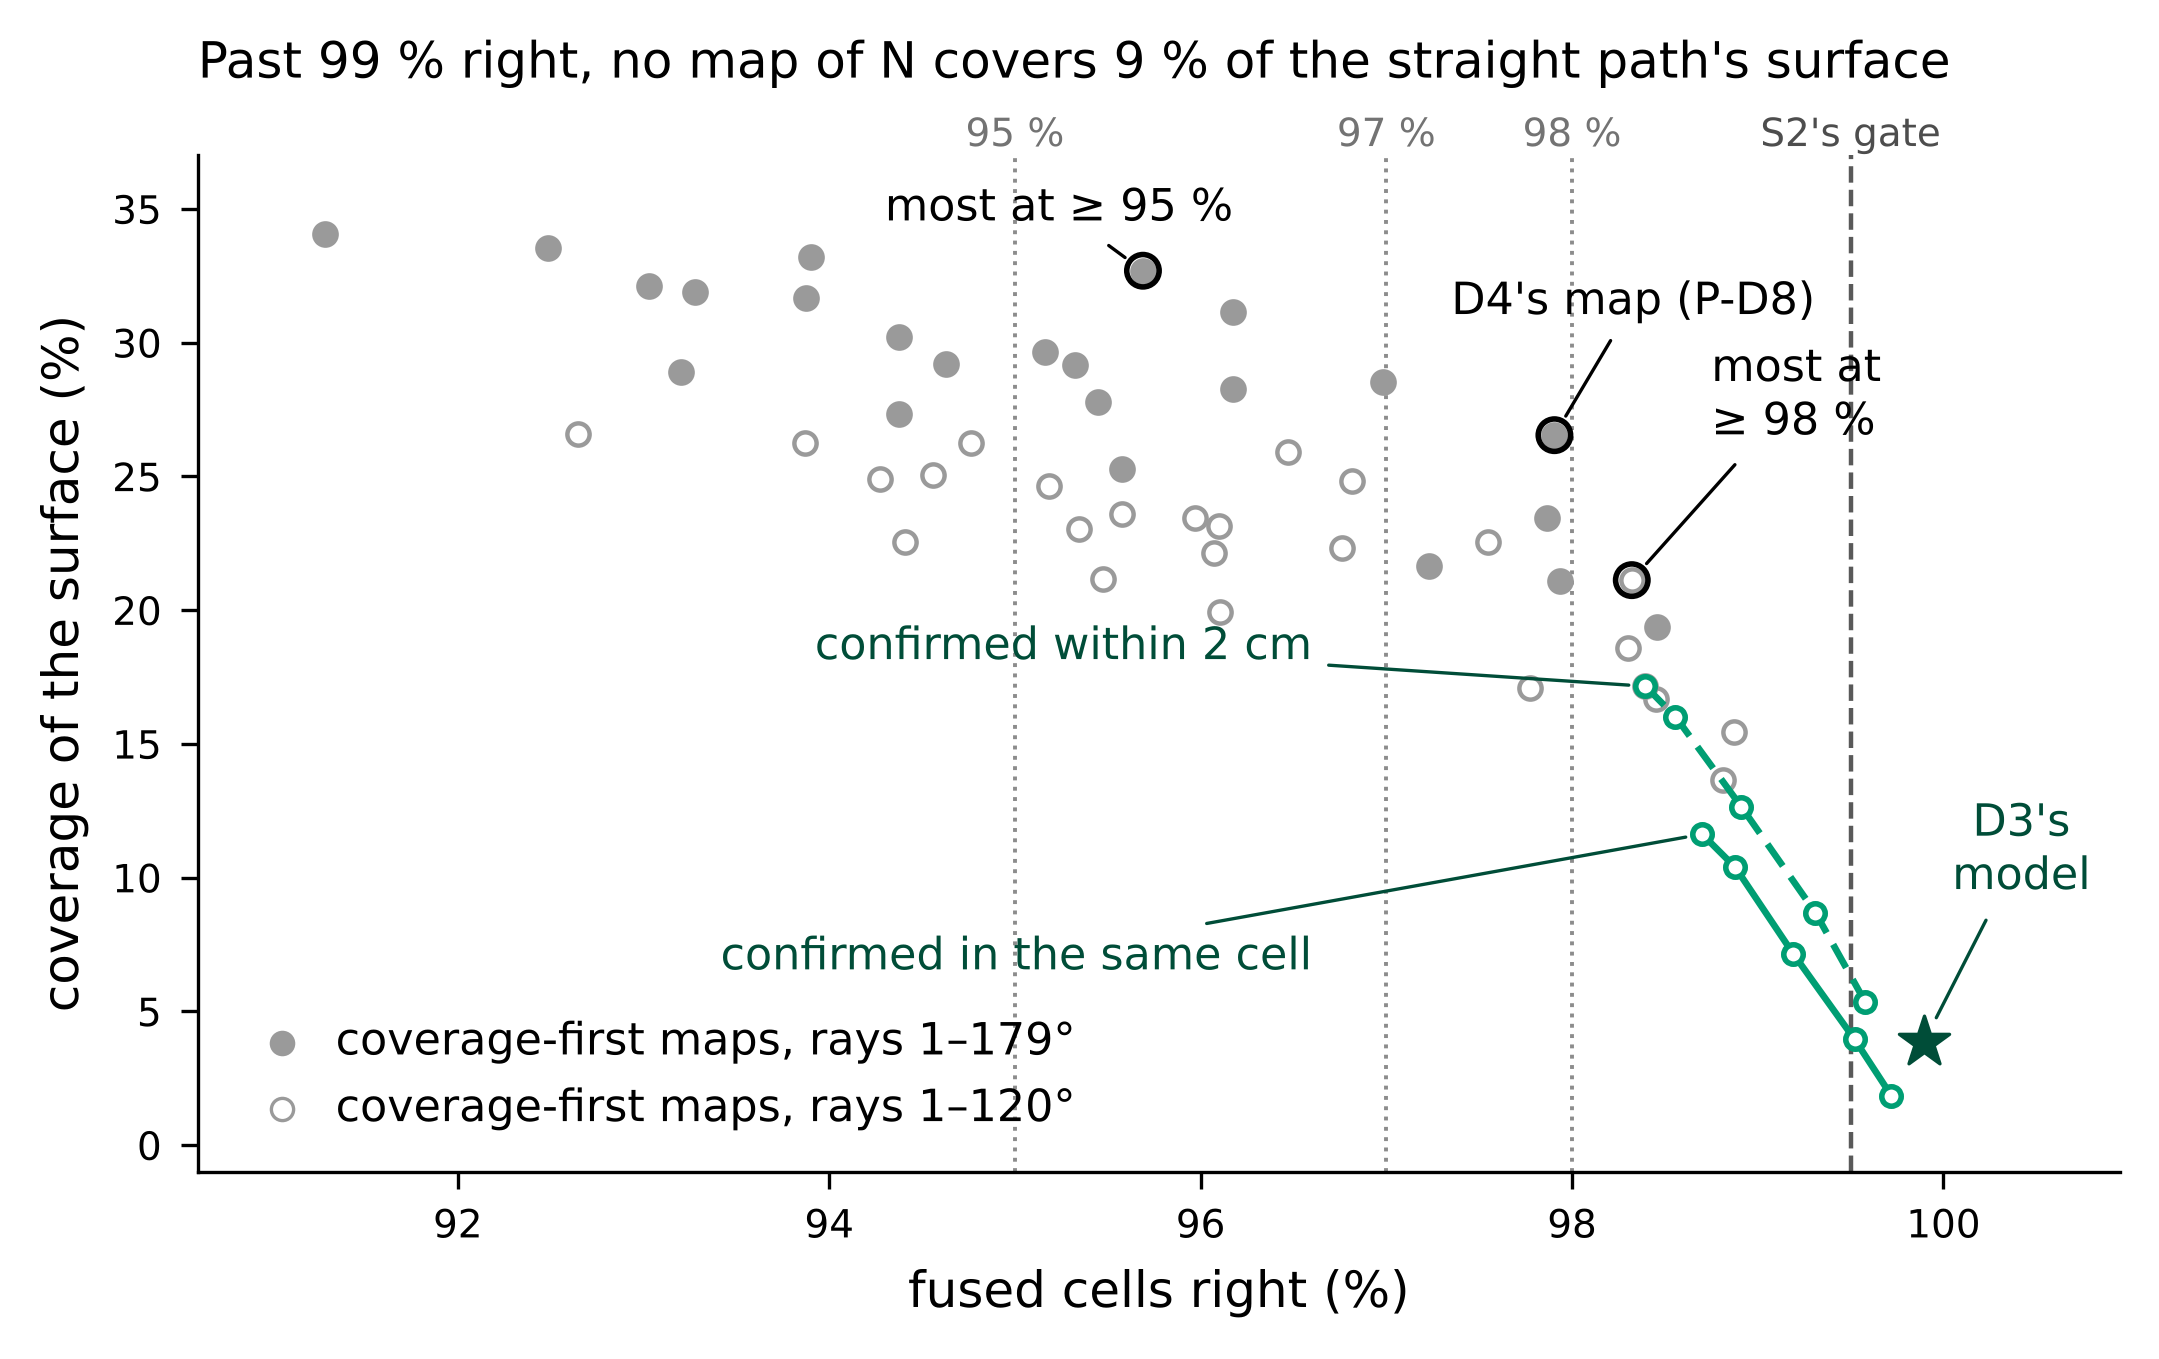
\includegraphics[width=\linewidth]{frontier.png}
\caption{Coverage against fused cells right on the straight path. Grey: stage 13a's 48 coverage-first maps, filled for the
rays 1--179$^\circ$ and open for 1--120$^\circ$; outlined, the map that covers most at each floor. Green: stage 12b's
confirmed models of N1024, with the span growing from 0\,m (upper left) to 1.0\,m (lower right) along each line. The
star: demo D3's model. The perfect matcher, at 99.98\,\% right and 80.4\,\% coverage, lies off the plot. Code,
workstation\WS; drawn in the Chat sandbox.}\label{fig:frontier}
\end{figure}

% ================================================================================================
\section{Coverage first}\label{sec:coverage}

D3's model covered too little to be useful, while every cell N reported, at 97.77\,\% right, seemed acceptable. Luiz
asked for the opposite test: how far can coverage be pushed within a usable reconstruction (P-D7, \#31)?

\paragraph{Stage 13a} built every map from the caches, with no new matching. It joined three things.
\begin{itemize}
\item \textbf{Six anchor sources:} N1024 as it is; N with the depth-edge tolerance at 10\,\% of $\zeta$, the diagnosis's
  alternative; N with the test off; the same with unsupported anchors readmitted (approximately); and N1024 or N at
  10\,\% joined with N on the short $\pm0.2$\,m windows (5 frames), whose estimates are fused with the long windows'.
\item \textbf{Two ray sets:} 1--179$^\circ$ and 1--120$^\circ$.
\item \textbf{Four truth-free filters:} none; at least one, or at least three, of the 26 cells around a cell also in the
  map; or an estimate of a second reference within 2\,cm.
\end{itemize}
That makes 48 maps (Figure~\ref{fig:frontier}), reported as a frontier: the map that covers most at each floor of cells
right (Table~\ref{tab:frontier}).

\begin{table}[h]
\centering\small
\begin{tabularx}{\linewidth}{@{}lcLrcr@{}}
\toprule
floor & coverage & the map & cells & right & gross\\
\midrule
98\,\% & 21.1\,\% & N1024 + N on $\pm0.2$\,m windows, rays 1--120$^\circ$, $\ge3$ neighbours & 218,153 & 98.32\,\% & 2,244\\
97\,\% & 26.5\,\% & N1024 + N on $\pm0.2$\,m windows, rays 1--179$^\circ$, $\ge3$ neighbours & 284,561 & 97.91\,\% & 3,679\\
95\,\% & 32.7\,\% & N at 10\,\% + N on $\pm0.2$\,m windows, rays 1--179$^\circ$, $\ge1$ neighbour & 414,800 & 95.69\,\% & 9,841\\
\bottomrule
\end{tabularx}
\caption{Stage 13a's frontier on the straight path. Gross: cells more than 25\,\% off in range. For scale, the perfect
matcher covers 80.4\,\%, and 39.7\,\% where the gradient's signal-to-noise ratio is at least 3. Code,
workstation\WS{} (\code{stage13a.json}).}\label{tab:frontier}
\end{table}

\paragraph{The middle ground.} Luiz set the usable floor at 97\,\% right and took the map that covers most there:
N1024 joined with N on $\pm0.2$\,m windows, rays 1--179$^\circ$, cells with at least 3 neighbours (P-D8). The filter
needs no truth and no second reference: an isolated cell is dropped. \textbf{Demo D4} (\#32) grew this map along the
straight path. It ended at 284,561 cells, 97.91\,\% right, 26.5\,\% coverage, equal to stage 13a's batch map, and 1.55
times the coverage of D3's every cell\WS. By sector it is 99.03\,\% right in 0--15$^\circ$ and 99.08\,\% in
15--60$^\circ$, but 96.75\,\% in 60--120$^\circ$ and 96.49\,\% in 120--165$^\circ$ (Figure~\ref{fig:tour}c). Like D3,
it was chosen on the data it shows.

% ================================================================================================
\section{N on curved paths}\label{sec:arcs}

To validate P-D8's settings, Luiz chose to redo demo D2 on the Classroom's L-tour (P-D9): the straight path's first
2\,m, then the turn, which is 0.3\,m of line, a quarter arc of radius 1\,m to the left, and 0.3\,m of line. On that tour,
18 of the 32 references have windows that reach the arc, and N refused them. The other 14 lie where the settings were
chosen. So N had to work on arcs first (stage 14, \#34). This is also the project's own aim, depth along curved paths.

\paragraph{Where the line was assumed.} Only N's coarse search needs a line. It unwraps the reference and every frame
into one pencil of planes about the path's line. There a static point at inverse range $\zeta$ keeps its plane and moves
along it from $\psi$ to
\begin{equation}
\psi'_k=\operatorname{atan2}\left(\sin\psi,\ \cos\psi-t_k\zeta\right),\label{eq:shift}
\end{equation}
with $t_k$ the frame's signed distance along the line. The fine fit already projects each patch sample through each
frame's exact pose. One more quantity assumed the line: the pixels per unit of $\zeta$, $t_{\max}\sin\psi/\text{res}$,
which set the coarse step, the peak exclusion, the fit's move limit, and the support and depth-edge tests.

\paragraph{One pencil per frame.} For frame $k$, the baseline from the reference $c_r$ is $c_k-c_r=t_k e_k$, with
$t_k>0$ and $e_k$ a unit vector. The reference and frame $k$ are both sampled on the pencil about $e_k$, by world
direction, so the frame's rotation is undone exactly. In that pencil the motion is a pure translation, and
Equation~\ref{eq:shift} holds with $\psi$ measured from $e_k$. Each anchor's curve for frame $k$ is read at its own row
and column of that frame's grid, and the curves are averaged over the frames as before. The pixels per unit of $\zeta$
become, per anchor, $\max_k t_k\sin\angle(u,e_k)/\text{res}$, for the anchor's ray $u$. On a line every $e_k$ is $\pm h$,
the heading, and the per-frame grids are N's own, mirrored for the frames behind. The fine fit, the patch, every
threshold imported from M4, and the line's code path are unchanged. The per-frame path runs only where the line's test
fails, or when it is forced, as in check G0.

On an arc of radius $R$, the chord to a frame $s$ ahead turns by $s/2R$ from the tangent, and the head itself by $s/R$.
On the 1\,m turn, over $\pm0.5$\,m, the baselines spread over $\pm14.3^\circ$ and the head turns by up to $28.6^\circ$
(computed; Figure~\ref{fig:pencils}b).

\begin{figure}[t]
\centering
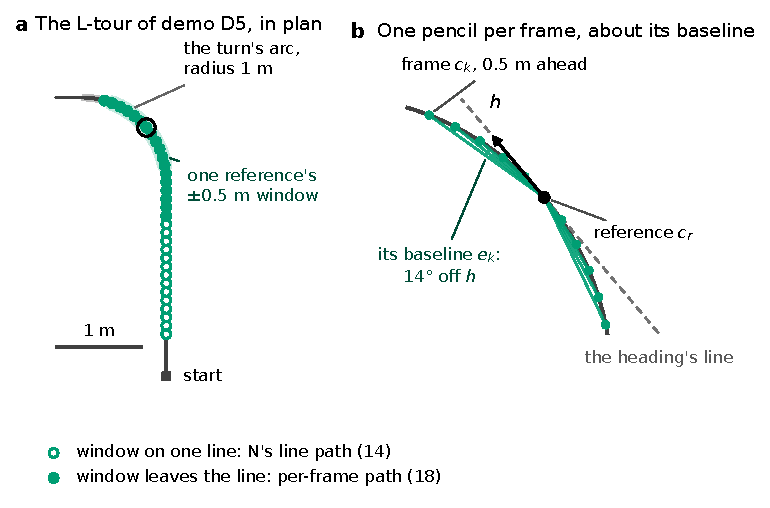
\includegraphics[width=\linewidth]{tour_pencils.pdf}
\caption{(a) Demo D5's L-tour, in its own frame: references every 10 looks, open where the reference's $\pm0.5$\,m
window lies on one line and N takes its line path, filled where the window leaves the line and N takes its per-frame
path (from \code{demo5.json}). (b) The reference ringed in (a), on the arc, with its ten frames over $\pm0.5$\,m: each
frame's pencil is about its own baseline $e_k$, which turns from the heading $h$ by half the arc between them. Drawn to
scale in the Chat sandbox.}\label{fig:pencils}
\end{figure}

\paragraph{The checks} were declared before data, each with a control that must fail (Table~\ref{tab:checks14}).

\begin{table}[h]
\centering\small
\begin{tabularx}{\linewidth}{@{}lLLl@{}}
\toprule
check & what it says & control (must fail) & result\\
\midrule
G0 & The per-frame path forced on the straight path gives N back: $\ge99.9$\,\% same decisions, the accepted $\zeta$ to
$10^{-9}$ relative, cells right and coverage to 0.05 points & the per-frame path with the mirrored path's poses &
\textbf{fails on $\zeta$}\WS\\
G1 & M4's fixtures, rendered along an arc of radius 1.0\,m, pass M4's gates & steps 20\,\% long; the poses of a 1.2\,m
radius; the scene scaled $1.5\times$ & passes\SB\\
G2 & On R3's turn at 1024 spp, N covers at least twice B1024's coverage, at cells right at most 2 points below B1024's
& N with the mirrored path's poses & passes\WS\\
C0 & B at 128 spp and the perfect matcher reproduce stage 9's turn numbers & B on the 1024-spp renders & passes\WS\\
\bottomrule
\end{tabularx}
\caption{The checks of stage 14 (\#34). Every control fails as it must. M4's gates: median $\le0.1$\,px, 90th percentile
$\le0.25$\,px, at least 100 accepted, and on the periodic fixture at most 1\,\% over 1\,px. C1's radial fixture was
dropped, since its texture is constant along a line's traces but not along an arc's.}\label{tab:checks14}
\end{table}

\paragraph{The fixtures (G1).} Along the arc, the front plane is 96.6\,\% accepted at a median error of 0.033\,px; the
tilted plane 60.0\,\% at 0.037\,px; the corridor's parallel wall 42.1\,\% at 0.030\,px; the periodic texture has no
accepted anchor over 1\,px\SB. The controls fail as they must: with steps 20\,\% long, 0.3\,\% are accepted at a median
of 12\,px; with a 1.2\,m radius, 0.06\,\% at 7.7\,px; with the scene scaled, 96.1\,\% are accepted, but at 3.5\,px.

\paragraph{The turn (G2).} At its 12 references, every one of whose windows reaches the arc, N covers 26.61\,\% at
98.24\,\% right, against 13.12\,\% at 94.07\,\% for B1024, the M\"obius Traces note's sweep B on the same
renders\WS. Its control accepts 38 cells, none right. Table~\ref{tab:turn}
sets N on the turn beside N on the straight path, by sector. On the turn it covers more and is more often right overall,
and more often right in every sector but the thin 165--180$^\circ$. The two paths see different surfaces, though: the perfect matcher covers
86.15\,\% on the turn and 80.37\,\% on the straight path.

\begin{table}[h]
\centering\small
\begin{tabular}{@{}lrcrc@{}}
\toprule
 & \multicolumn{2}{c}{straight path} & \multicolumn{2}{c}{turn}\\
\cmidrule(lr){2-3}\cmidrule(lr){4-5}
sector & cells & right & cells & right\\
\midrule
all & 179,823 & 97.23\,\% & 120,463 & 98.24\,\%\\
0--15$^\circ$ & 18,851 & 94.02 & 3,844 & 99.04\\
15--60$^\circ$ & 79,687 & 98.94 & 50,733 & 99.33\\
60--120$^\circ$ & 35,881 & 97.18 & 41,522 & 97.76\\
120--165$^\circ$ & 40,430 & 95.68 & 23,063 & 96.97\\
165--180$^\circ$ & 4,974 & 95.01 & 1,301 & 91.78\\
\midrule
coverage & & 21.63\,\% & & 26.61\,\%\\
\bottomrule
\end{tabular}
\caption{N1024 on the straight path (its line path) and on the turn (its per-frame path), every cell, rays
1--179$^\circ$, 12 references each. Code, workstation\WS{} (\code{stage13a.json} and \code{stage14.json}).}\label{tab:turn}
\end{table}

\paragraph{No regression on the line (G0).} Forced onto the straight path, the per-frame path takes the same decision as
N's line path for 2,345,468 of 2,345,469 anchors. The fused maps agree: 179,823 and 179,824 cells, 97.2317 and
97.2312\,\% right, the same coverage\WS. Of the 301,581 anchors both accept, 301,547 have bit-identical $\zeta$, but three
differ by more than $10^{-9}$ relative, up to $2.2\times10^{-8}$, about 0.04\,\textmu m at 2\,m (computed). So G0 fails on its $\zeta$
bound alone. Code showed that each path reproduces itself bit for bit, so the differences belong to the per-frame path.
For a frame behind the reference, its grid is N's mirrored, equal up to $6.9\times10^{-16}$ (Chat sandbox). The rest is
inferred, not measured: the coarse sums are taken in float32, so a last-bit difference sometimes rounds the other way;
the fine fit runs a fixed eight iterations, so part of the different start remains. The bound had been set from a single
CPU test where the two paths happened to agree bit for bit. It was not moved, and Luiz chose to go on with G0 recorded as
failed (P-D10).

% ================================================================================================
\section{The tour}\label{sec:tour}

\paragraph{Demo D5} (\#35) redoes demo D2~\cite{mobius}, which set the perfect matcher beside the real matcher of the
M\"obius Traces note, the sweep B with its seeded fill H, on the same L-tour: 418 looks, 4.17\,m, a reference every 10
looks (32 in all), each released when its window is complete, 0.5\,m behind the current look. One side shows D2's
perfect matcher, with D2's own draws. The other shows P-D8's coverage map, built from N on the 1024-spp renders, on each
reference's $\pm0.5$\,m and $\pm0.2$\,m windows. N takes its line path at the 14 references whose window lies on one line
and its per-frame path at the 18 whose window leaves it (Figure~\ref{fig:pencils}a). The match video draws every cell in
the scene's colour; an error video, as in D2, colours each by its error. Both maps are judged by stage 9's metric against
the 128-spp truth. The profile is S2's build profile, with five declared departures: the tour, the two window sets, the
neighbour filter in place of confirmation (hence no span), and the 97\,\% floor, with S2's 99.5\,\% gate reported only.

\paragraph{The checks} were declared before data. All pass, and every control fails\WS. The perfect side's end map equals
D2's to the last digit (V0). The tour is the planned curve, to $6\times10^{-16}$\,m (V2). Both end maps equal their batch
fusion (V3). Nothing is shown before its window is complete (V4). The error video's colours equal stage 9's verdicts
(C), and each PLY file, read back, holds exactly its map (P1). N with the mirrored path's poses gives 531 cells, none
right. The run took 26\,min on the workstation.

\begin{table}[h]
\centering\small
\begin{tabular}{@{}lrcrrc@{}}
\toprule
end of the tour & cells & right & wrong & gross & coverage\\
\midrule
the perfect matcher (D2's) & 649,153 & 99.97\,\% & 185 & 4 & 88.9\,\%\\
\textbf{N's coverage map} ($\ge3$ neighbours) & \textbf{600,922} & \textbf{97.67\,\%} & 13,979 & 7,785 & \textbf{38.1\,\%}\\
every cell N reported & 720,727 & 94.73\,\% & 37,979 & & 40.6\,\%\\
\midrule
D2's real matcher, B + H, on 128 spp & 1,008,509 & 73.6\,\% & 265,751 & & 41.4\,\%\\
\bottomrule
\end{tabular}
\caption{Demo D5's end maps, and D2's real matcher on the same tour. Gross: more than 25\,\% off in range. Code,
workstation\WS{} (\code{demo5.json}; D2's row from \code{demo2.json}, its wrong cells computed from its cells and cells
right).}\label{tab:d5}
\end{table}

\paragraph{The validation, declared before data: yes.} On the cells whose dominant reference's window leaves the line,
where N takes its per-frame path, data P-D8 was not chosen on, is the map at least 97\,\% right? It is 97.76\,\% right on
272,609 cells (6,094 wrong, 3,290 gross), against 97.60\,\% on the 328,313 cells from windows on one line (7,885 wrong,
4,495 gross)\WS. The 18 references are 190 to 360; the short window leaves the line at 15 of them, from 220 on.

\paragraph{The whole map} (Table~\ref{tab:d5}, Figures~\ref{fig:tour} to~\ref{fig:ply}) covers 38.1\,\% of the surface,
43\,\% of what the perfect matcher covers, at 97.67\,\% right, just under D4's 97.91\,\% on the straight path alone. From
the first release, at look 101, to the last, its cells right stay between 97.65 and 98.19\,\%. Against D2's real matcher
the coverage is about the same, 38.1 against 41.4\,\%, and the share of wrong cells falls from 26.4 to 2.3\,\%: 13,979
wrong cells against 265,751. D5 differs from D2 in three ways at once, though: the matcher (N against B + H), the renders
it matches (1024 against 128 spp) and the acceptance (the neighbour filter). The diagnosis found that the first two each
matter; D5 does not separate them.

\begin{figure}[t]
\centering
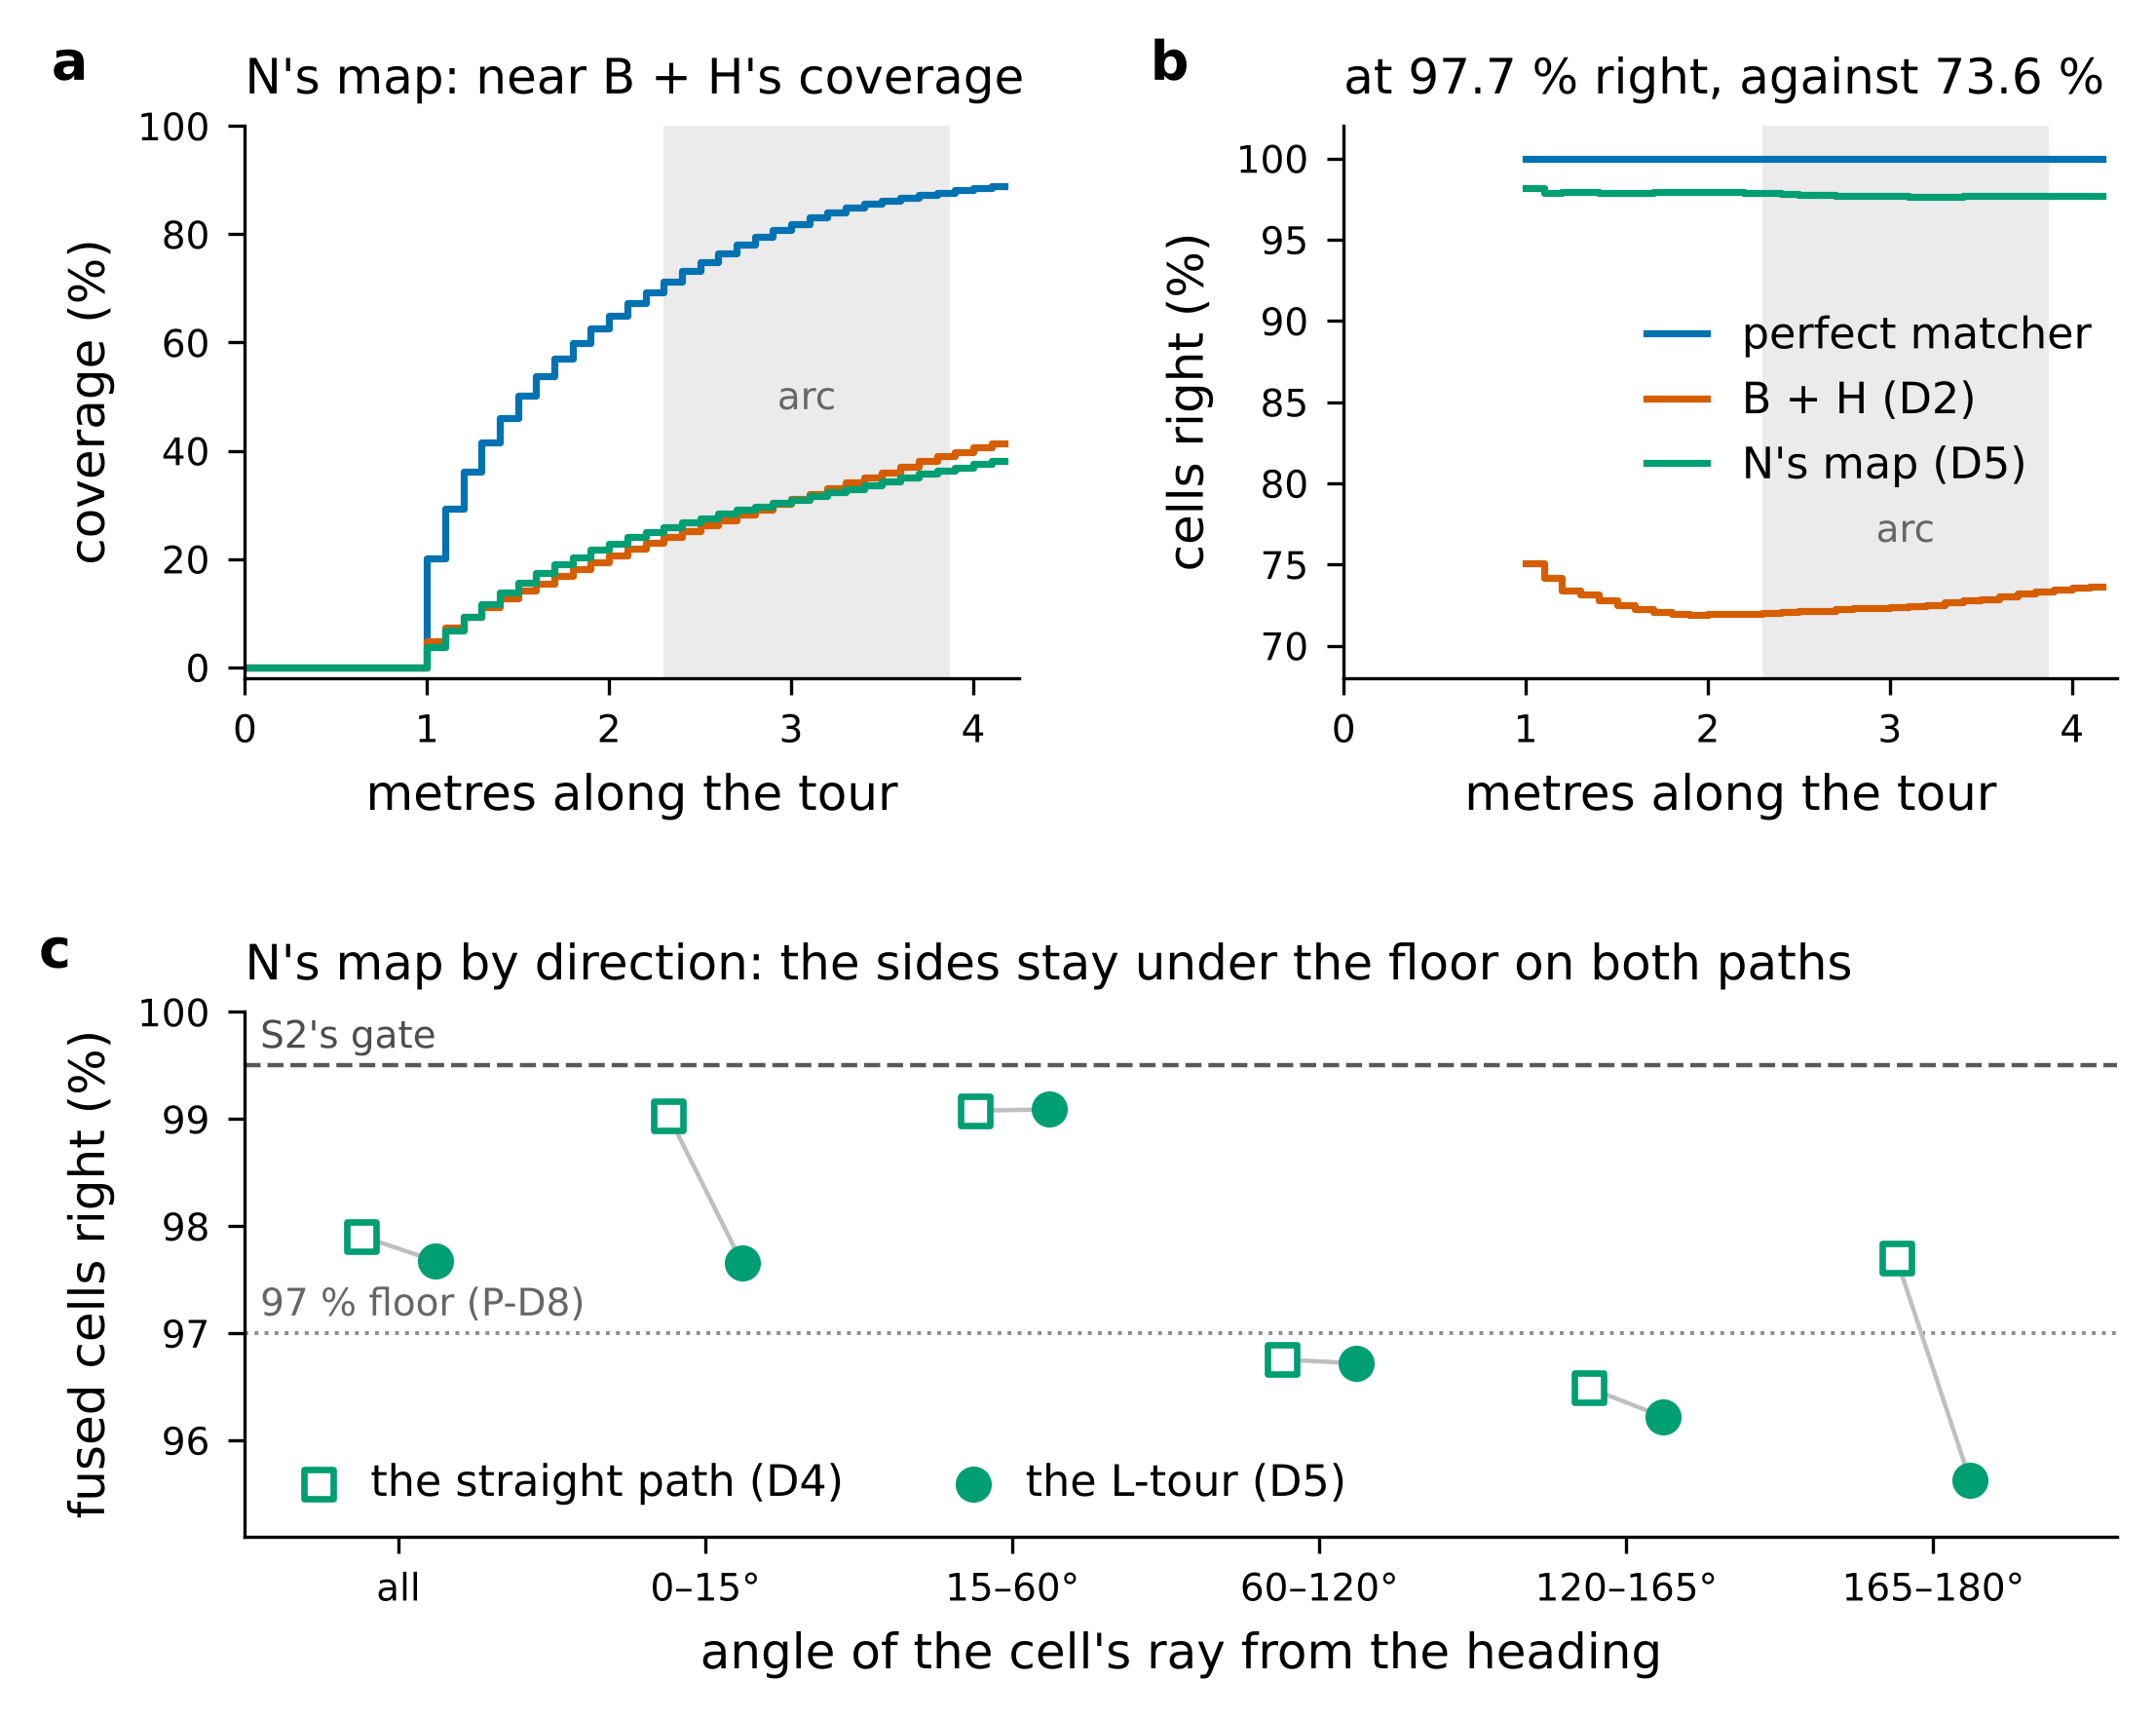
\includegraphics[width=\linewidth]{tour_curves.png}
\caption{(a, b) Along the L-tour, demo D2's perfect matcher and real matcher (B + H, on 128-spp renders) and demo D5's
coverage map (N, on 1024-spp renders): coverage of the surface and fused cells right. A reference's cells join the map
0.5\,m after it. Grey: the head is on the arc. (c) The coverage map's cells right by sector of the angle from the
heading, on the straight path (D4, 12 references) and on the tour (D5, 32 references). Code, workstation\WS; drawn in
the Chat sandbox.}\label{fig:tour}
\end{figure}

\paragraph{By sector} (Figure~\ref{fig:tour}c). The map is 99.09\,\% right in 15--60$^\circ$, on 258,551 cells, but
96.72\,\% in 60--120$^\circ$ and 96.22\,\% in 120--165$^\circ$, on 164,484 and 131,978 cells. These two side sectors hold
10,389 of the map's 13,979 wrong cells, 74\,\%. They sit just under 97\,\% on the straight path too. This is where the
diagnosis located N's weakness: near surfaces seen to the side change appearance over the window more than N's patch
model follows. Two sectors moved
between the straight path and the tour: 0--15$^\circ$, from 99.03 to 97.65\,\% (38,019 cells), and 165--180$^\circ$,
from 97.70 to 95.63\,\% (7,890 cells). On the turn alone, without the short windows or the filter, N was 99.04\,\% right in
0--15$^\circ$ (Table~\ref{tab:turn}). D5's record does not break the sectors down by segment or by window, so where the
loss near the heading comes from is not yet known.

\begin{figure}[t]
\centering
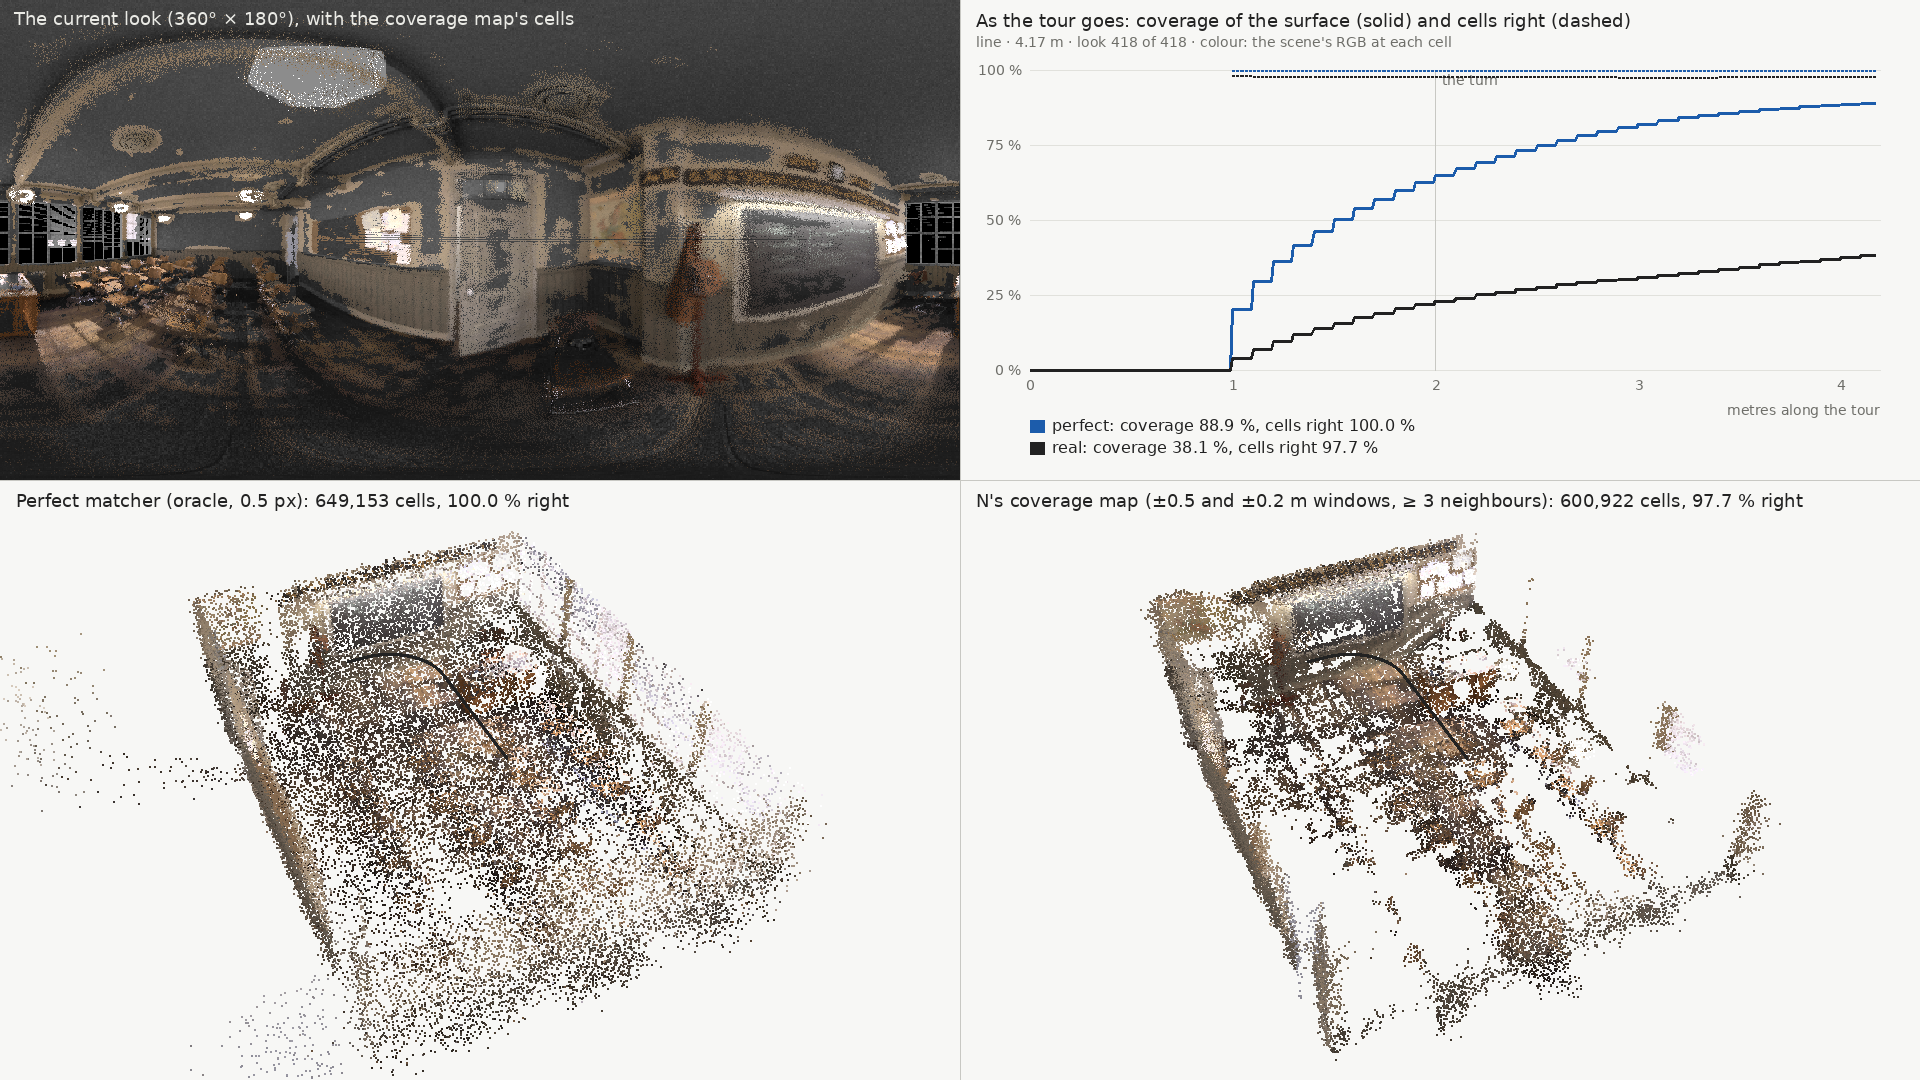
\includegraphics[width=\linewidth]{d5_last_match.png}
\caption{The last frame of demo D5's match video, unedited. Top: the current look, with the map's cells, and coverage
and cells right along the tour. Bottom: the perfect matcher's map (left) and N's coverage map (right), each cell in the
scene's colour; the black curve is the tour. Code, workstation\WS{} (\code{last\_match.png}).}\label{fig:frame}
\end{figure}

\begin{figure}[t]
\centering
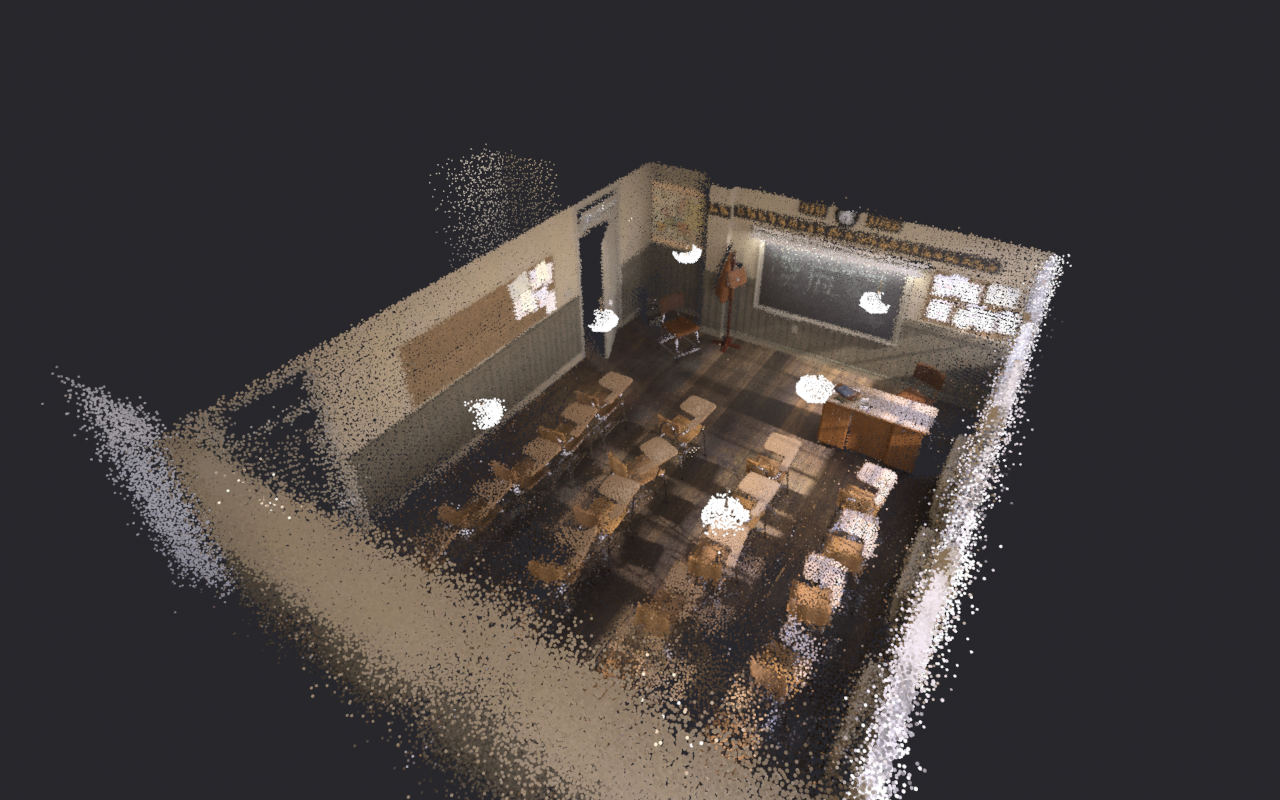
\includegraphics[width=0.329\linewidth]{classroom_tour_perfect.png}\hfill
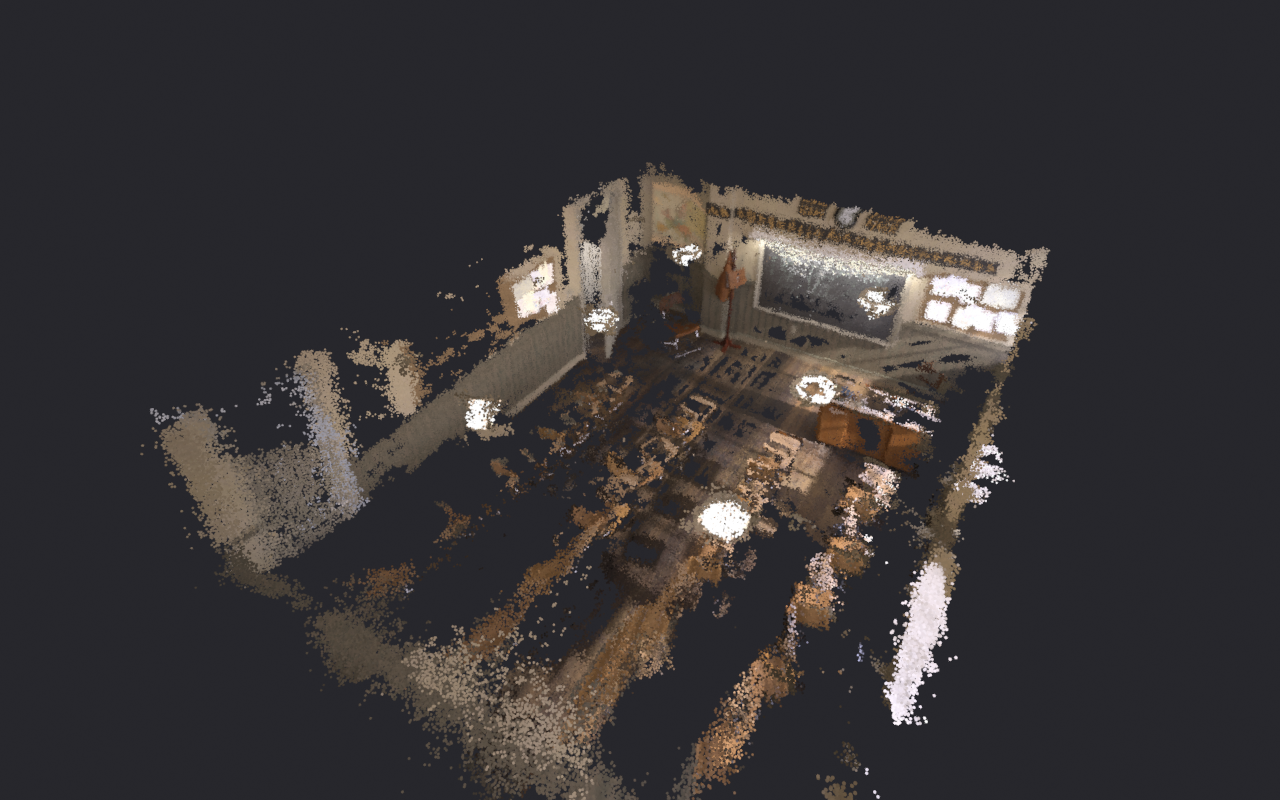
\includegraphics[width=0.329\linewidth]{classroom_tour_map.png}\hfill
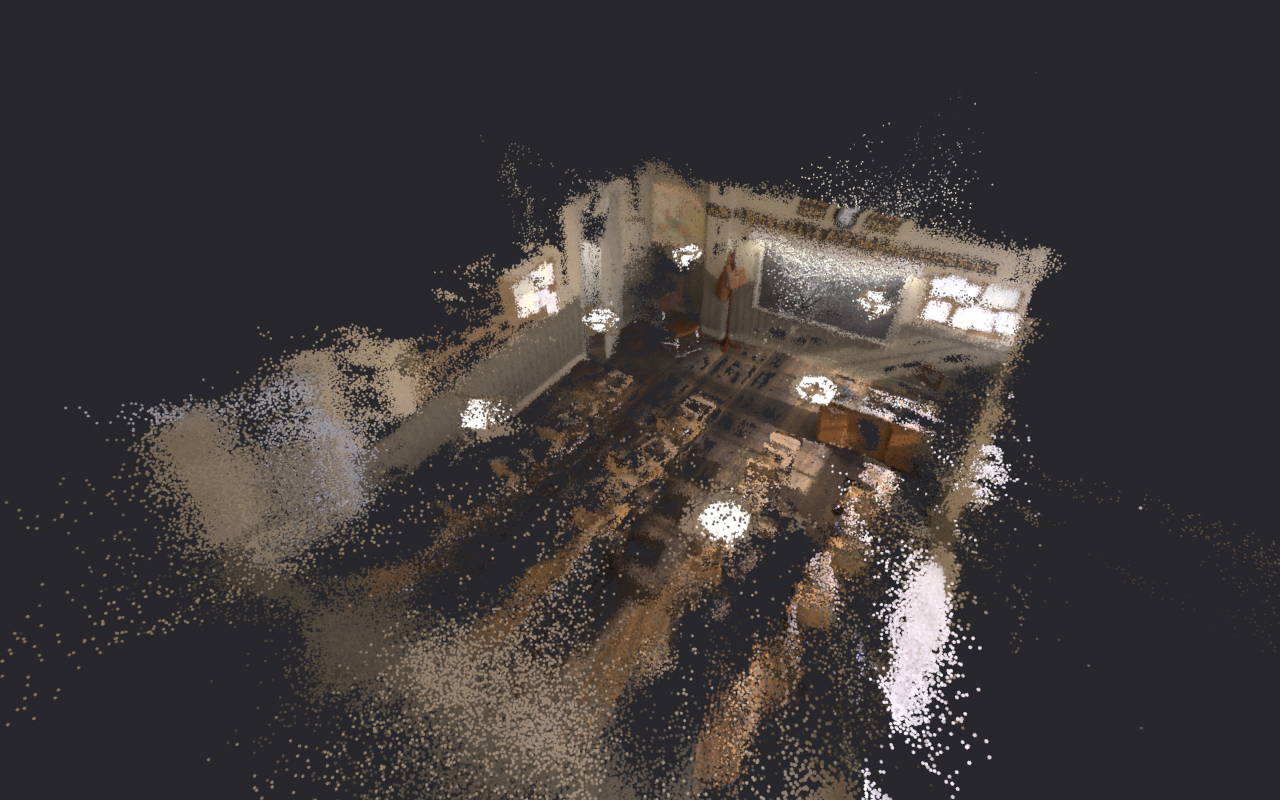
\includegraphics[width=0.329\linewidth]{classroom_tour_all.png}
\caption{D5's three PLY files from one camera: the perfect matcher (649,153 points), N's coverage map (600,922) and every
cell N reported (720,727). The neighbour filter removes the scattered cells around the room. Rendered in headless
Blender by Code, workstation\WS{} (\code{classroom\_tour\_\{perfect,map,all\}.png}).}\label{fig:ply}
\end{figure}

% ================================================================================================
\section{Conclusions}\label{sec:conclusions}

\begin{enumerate}
\item \textbf{Errors first, as S2 defines it, is too strict for N on this scene.} Past 99\,\% right, no map of the
  straight path covers 9\,\% of its surface. Confirmation removes errors and coverage together, and costs even the
  perfect matcher much of its coverage: 80.4\,\% falls to 29.8\,\% under S1's rule.
\item \textbf{Coverage first, with a truth-free filter, gives a usable map:} at the 97\,\% floor, 26.5\,\% of the
  straight path's surface at 97.91\,\% right.
\item \textbf{N works on curved paths.} One pencil per frame, about its baseline, makes the motion a pure translation
  again. On the Classroom's turn N covers 26.61\,\% at 98.24\,\% right, against 21.63\,\% at 97.23\,\% on the straight
  path.
\item \textbf{The settings hold off the line.} On the tour, the map is 97.76\,\% right where N's windows leave the line,
  against 97.60\,\% on the line. The whole map covers 38.1\,\% at 97.67\,\% right, where D2's real matcher covered 41.4\,\%
  at 73.6\,\%.
\item \textbf{The side of the field does not move.} Rays 60--165$^\circ$ from the heading stay just under 97\,\% on both
  paths and hold three quarters of the tour's wrong cells.
\end{enumerate}

% ================================================================================================
\section{What remains}\label{sec:remains}

\begin{itemize}
\item \textbf{The sides.} The diagnosis proposed patches warped fully by the hypothesis (slopes along and across the
  trace), windows suited to each ray's parallax, short for near lateral points, and more frames against noise. The
  measured target is now plain: 60--165$^\circ$ from 96.2--96.7\,\% to above 97\,\%, and then toward S2's 99.5\,\%.
\item \textbf{The heading's sectors on the tour.} 0--15$^\circ$ and 165--180$^\circ$ lost 1.4 and 2.1 points between
  D4 and D5. A breakdown of D5's map by sector, segment and window, from its caches, would say why before anything is
  changed.
\item \textbf{One scene, one turn.} The settings were chosen on the Classroom's straight path and validated on the same
  room's turn. Another scene, a pivot or a tighter arc would test them further. So would the standard's open item,
  a noise target set in signal-to-noise ratio rather than in samples per pixel.
\item \textbf{Errors first, later.} The confirmed model is still the aim of an incremental build. With N at 97--98\,\%
  right, it needs more evidence to confirm from: a longer path, more references, or rays chosen where N is reliable.
\item \textbf{A lesson for checks.} G0's bound asked for agreement to $10^{-9}$ between two computations whose float32
  sums need not agree bit for bit. A bound on numerical agreement should come from the arithmetic it compares, not from
  one test that happened to agree exactly.
\end{itemize}

% ================================================================================================
\section{How the work was done}\label{sec:process}

As before, the N-Surface method~\cite{nsurface} in its light form. Claude in a chat sandbox (``Chat'') planned, wrote
the code and its checks, and ran what a CPU can: the fixtures along an arc, and dry runs on synthetic rooms and on the
calibration room's tour. Claude Code on the RTX~4090 workstation (``Code'') rendered the turn at 1024 spp (10\,min
38\,s) and ran the Classroom. Luiz accepted the standard, delegated one choice (``pick the option that gives the best
result''), set the usable floor, chose to validate on the tour and to extend N to arcs first, and chose to go on with G0
failed. Every check was declared before data, with a control that must fail.

The standard earned its place on the first day. Its \code{check\_record} caught a missing control in G1 and an
undeclared departure in D5's dry run. A stamp key that overwrote a harness's own was fixed at its cause.
Two checks were Chat's mistakes, owned in their issues and left as declared: stage 12's check on sectors too thin to
judge, which led to S2, and G0's bound. When the calibration room's reference render turned out not to be on the
workstation, Code replaced D5's dry run with a smoke test on the real tour and declared the change before data. Chat
re-rendered the reference in the sandbox and ran the dry run there in parallel. All of this took one day,
21 November 2026; D5 finished late that night.

\paragraph{Records.} Everything above is in \code{visgraf/deep-motion}~\cite{dm}, on \code{main} at \code{190332a}:
\pth{docs/standard.md}; \pth{docs/plan.md} (decisions P-D4 to P-D10, and the results of stage 14 and demo D5); issues
\#27 to \#35; and the records in \pth{docs/runs/dm-issue-28/} (stages 12 and 12b), \pth{dm-issue-29/} (D3),
\pth{dm-issue-31/} (stage 13a), \pth{dm-issue-32/} (D4), \pth{dm-issue-34/} (stage 14, G1, G0's diagnostics) and
\pth{dm-issue-35/} (D5). The videos and PLY files stay on the workstation. Figure sources are listed in
\pth{figs/SOURCES.md}.

% ================================================================================================
\begin{thebibliography}{99}
\bibitem{dm} VISGRAF Lab. \emph{deep-motion}: depth from motion along curved paths.
  \url{https://github.com/visgraf/deep-motion}
\bibitem{diag} Luiz Velho and Claude. ``Why the Real Matcher Fell Short: A Diagnosis on a Straight Path''. VISGRAF
  technical note, 21 November 2026. \url{https://github.com/lvelho/foveal-depth-tr}
\bibitem{mobius} Luiz Velho and Claude. ``M\"obius Traces: Depth from Motion along Curved Paths''. VISGRAF technical note,
  20 November 2026. \url{https://github.com/lvelho/foveal-depth-tr}
\bibitem{tr2} Luiz Velho and Claude. ``Foveated Vision on a Moving Head: Depth from Forward Motion''. VISGRAF technical
  note, 15 November 2026. \url{https://github.com/lvelho/foveal-depth-tr}
\bibitem{nsurface} Luiz Velho and Claude. ``The N-Surface Method: Rigor and Spontaneity in Human--AI Research''.
  VISGRAF technical note, 2026.
\end{thebibliography}

\end{document}
